\subsection{李子代数的包络代数}

设 g 是 K 上的李代数，h 是 g 的子代数，\(\sigma\)、\(\sigma'\) 分别是 g、h 到其包络代数 U、V 的典范映射。于是 h 到 g 的典范嵌入 i 定义了一个从 V 到 U 的同态 i，称为典范同态，并满足 \(\sigma \circ i = i \circ \sigma'\)。代数 \(i(\mathrm{V})\) 由 1 和 \(\sigma(\mathfrak{h})\) 生成。我们将看到（第 7 号，定理 5 的推论），在重要的情形中 i 是单射。

若 \(\mathfrak{h}\) 是 \(\mathfrak{g}\) 的理想，则由 \(\sigma(\mathfrak{h})\) 生成的 U 的左理想与由 \(\sigma(\mathfrak{h})\) 生成的右理想相同，换言之，它是双边理想 R。这是因为对 \(x \in \mathfrak{h}\) 和 \(x' \in \mathfrak{g}\)，

\[
\sigma (x) \sigma (x ^ {\prime}) = \sigma (x ^ {\prime}) \sigma (x) + \sigma ([ x, x ^ {\prime} ])
\]

且 \([x, x'] \in \mathfrak{h}\)。

命题 3. 设 \(\mathfrak{h}\) 是一个理想，并令 \(\mathfrak{g}, p\) 分别表示一个李代数及其典范满同态；该同态从 \(\mathfrak{g}\) 到 \(\mathfrak{g} / \mathfrak{h}\)，W 是 \(\mathfrak{g} / \mathfrak{h}\) 的包络代数。同态：

\[
\tilde {p}: \mathrm{U} \rightarrow \mathrm{W}
\]

由 \(p\) 典范定义的映射是满射，其核是理想 \(R\)，位于 \(U\) 中，并由 \(\sigma(h)\) 生成。

令 \(\sigma''\) 为从 \(g/h\) 到 W 的典范映射。交换图：

\pandocbounded{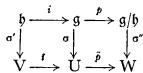
\includegraphics[keepaspectratio]{images/part001_4ab4ddcc.jpg}}

表明 \(\tilde{p}\) 在 \(\sigma(\mathfrak{h})\) 上为零，从而在 R 上为零。令 \(\psi\) 为从 U 到 U/R 的典范满同态。存在从 U/R 到 W 的同态 \(\phi\)

\pandocbounded{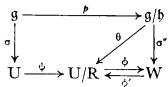
\includegraphics[keepaspectratio]{images/part001_c6a5c19d.jpg}}

到 W，使 \(\tilde{p} = \phi \circ \psi\)。映射 \(\psi \circ \sigma\) 把 \(g\) 映到 U/R，是一个 \(\alpha\)-映射，并且在 \(h\) 上为零，因而定义了一个 \(\alpha\)-映射 \(\theta\)，从 \(g / h\) 到 U/R，满足 \(\theta \circ p = \psi \circ \sigma\)。于是 \(\phi \circ \theta \circ p = \phi \circ \psi \circ \sigma = \sigma'' \circ p\)，所以 \(\phi \circ \theta = \sigma''\)。存在唯一的将 1 映到 1 的从 W 到 U/R 的同态 \(\phi'\)（第 1 号，命题 1），使 \(\theta = \phi' \circ \sigma''\)。于是 \(\phi' \circ \phi \circ \theta = \phi' \circ \sigma'' = \theta\)，且 \(\phi \circ \phi' \circ \sigma'' = \phi \circ \theta = \sigma''\)，因此 \(\phi' \circ \phi\) 和 \(\phi \circ \phi'\) 分别是 U/R 和 W 的恒等映射。证毕。

U/R 在同构 \(\phi\) 下与 W 相同。于是典范映射 \(\sigma''\) 将 \(g/h\) 映到 W，并与 \(\theta\) 相同，也就是与由取商后得到的将 \(g/h\) 映到 U/R 的映射 \(\sigma\) 相同。

